%===============================================================================
% DOCUMENT
%===============================================================================

%% Document class
\documentclass[a4paper,12pt]{scrreprt}

%% Include packages
\usepackage{packages}

\begin{document}

%% Include custom commands
\include{commands}

\pagenumbering{gobble}

%% Build cover
\definecolor{titlepagecolor}{RGB}{37,64,56}

%==========================================================================
% COLORED BAR ON THE LEFT SIDE
%==========================================================================

\backgroundsetup{
    scale=1,
    angle=0,
    opacity=1,
    contents={
        \begin{tikzpicture}[remember picture,overlay]
            \path [fill=titlepagecolor] (-10.5,-15) rectangle ++ (5,30);
            \node[color=white] at (-6.90,-11.5) {\bfseries {\fontsize{120}{60} \textsf{C}}};
            \node[color=titlepagecolor] at (-4.30,-11.5) {\bfseries {\fontsize{120}{60} \textsf{C}}};
        \end{tikzpicture}
    }
}

%==========================================================================
% COVER PAGE CONTENT
%==========================================================================

\title{\LARGE{Network Monitoring System}}

\author{
    Flávia Alexandra da Silva Araújo (A96587)\\ \quad
    Joshua David Amaral Moreira (A105684)\\ \quad
    Miguel Torres Carvalho (A95485)\\ \quad
}

%% Date
\date{\today}

%% Course
\newcommand{\Course}{Licenciatura em Engenharia Informática}

%% Department
\newcommand{\Department}{Escola de Engenharia}

%% UniName
\newcommand{\UniName}{Universidade do Minho}

%% UniPic
\newcommand{\UniPic}{
\includegraphics[width=120pt]{img/eeum.png}}

%% University
\newcommand{\University}{
    \begin{flushleft}
        \UniPic
    \end{flushleft}
    \textcolor{gray}{\small\textbf{\textsf{\UniName}}}\par
    \textcolor{gray!80!white}{\small{\textsf{\Department}}}\par
    \textcolor{gray!70!white}{\small{\textsf{\Course}}}
}

%% UC
\newcommand{\UC}{
    \begin{flushleft}
        \par\textcolor{titlepagecolor}{\Large\textbf{\textsf{Comunicações por Computador}}}
    \end{flushleft}
}

%% Project Phase
\newcommand{\SubTitle}{
    \begin{flushleft}
        \large\textbf{Trabalho Prático 2}
    \end{flushleft}
}

%% Group Info
\newcommand{\GroupInfo}{\par Grupo 10 - PL1}

%% GitHub Repo
\newcommand{\GitHubRepo}{\par\url{https://github.com/migueltc13/CC-tp2}}

%% School Year
\newcommand{\SchoolYear}{
    \par\small{\textsf{Ano Letivo de 2024/2025}}
}

%% Define new command to show title, author and date
\makeatletter
\let\Title\@title
\let\Author\@author
\let\Date\@date
\makeatother

%==========================================================================
% BEGIN COVER PAGE
%==========================================================================

%% Make cover page
\newcommand{\makecover}{

%% Removes page number on footer
\thispagestyle{empty}

%% No indentation
\setlength{\parindent}{0em}

%% Put Background defined on \backgroundsetup, in this page
\BgThispage

%% Changing geometry to prevent overlay with text
%% At the end of back cover, geometry is default with \restoregeometry
\newgeometry{top=4cm,left=6cm,right=2cm,bottom=2cm}

%% builds university info defined previously
\University
\vspace{1cm}
\UC
\SubTitle
\SchoolYear

\vspace*{4cm}
%% bigger space (i think its the default one) between paragraphs
\setlength{\parskip}{1em}

%% builds title info defined previously
\par\textbf{\textsf{\huge\Title}}
\vspace{1cm}
%% builds author(s) info defined previously
\par\Author

\vspace{0.5cm}

%% builds date info defined previously
\par\Date
\restoregeometry
\pagebreak

}

%==========================================================================
% END COVER PAGE
%==========================================================================

\makecover

%% Default geometry
\newgeometry{top=3cm,left=3cm,right=3cm,bottom=4cm}

%% Save default geometry
\savegeometry{default}

%% Load default geometry with:
% \loadgeometry{default}

%===============================================================================
% BEGIN ABSTRACT PAGE
%===============================================================================

\renewenvironment{abstract}
 {\par\noindent\textbf{\Large\abstractname}\par\bigskip}
 {}

\begin{flushleft}
\begin{abstract}
    \par No presente relatório, é apresentada a solução desenvolvida para a Unidade Curricular
    de \textbf{Comunicações por Computador}, como parte do projeto final do semestre -
    \textbf{\textit{Network Monitoring System}}.
    Este trabalho teve como objetivo projetar um sistema capaz de monitorizar
    o tráfego de rede, bem como o desempenho dos dispositivos, entre um servidor
    centralizado e vários agentes distribuídos, permitindo a execução de tarefas
    de monitorização, com a respetiva recolha de métricas de desempenho e envio
    de alertas previamente configurados.
    Adicionalmente, foi desenvolvida a análise de dados recolhidos e a apresentação
    dos mesmos em formato gráfico, permitindo a visualização do desempenho da rede
    e dos dispositivos monitorizados.

    No sistema desenvolvido implementaram-se dois protocolos aplicacionais: \\
    \textbf{\textit{AlertFlow}}:
    destinado ao envio de alertas quando certas condições de monitorização
    definidas são excedidas, utilizando, como protocolo de transporte,
    o \textit{Transmission Control Protocol} (TCP). \\
    \textbf{\textit{NetTask}}: implementado para a comunicação de tarefas de monitorização
    e recolha de métricas, sobre o \textit{User Datagram Protocol} (UDP),
    este protocolo aplicacional foi desenvolvido de forma a assegurar
    a comunicação robusta e confiável entre o servidor e os agentes.

    O trabalho foi concluído com a implementação e validação das principais funcionalidades do sistema,
    demonstrando a sua eficácia em ambientes de teste representativos em ambientes virtualizados.
    Este relatório documenta detalhadamente o \textit{design}, implementação, utilização
    e resultados obtidos.

\par \textbf{Palavras-Chave}: \textit{Network Monitoring System}, TCP, UDP,
    \textit{AlertFlow}, \textit{NetTask}, \textit{python3}, \textit{iperf3},
    \textit{ping}, \textit{Comunicações por Computador}.
\end{abstract}
\end{flushleft}

\pagebreak

%===============================================================================
% END ABSTRACT PAGE
%===============================================================================

%===============================================================================
% BEGIN INDEXES PAGES
%===============================================================================

%% Changes table of content name
\renewcommand{\contentsname}{Índice}
\renewcommand{\listfigurename}{Índice de Figuras}
\renewcommand{\lstlistlistingname}{Índice de \textit{Snippets}}

\tableofcontents
\pagebreak

\listoffigures
\pagebreak

\lstlistoflistings
\pagebreak

%===============================================================================
% END INDEXES PAGES
%===============================================================================

\pagenumbering{arabic}

%===============================================================================
% BEGIN ARQUITETURA DA SOLUÇÃO
%===============================================================================

\chapter{Arquitetura da Solução}

\begin{minipage}{\textwidth}
    \centering
    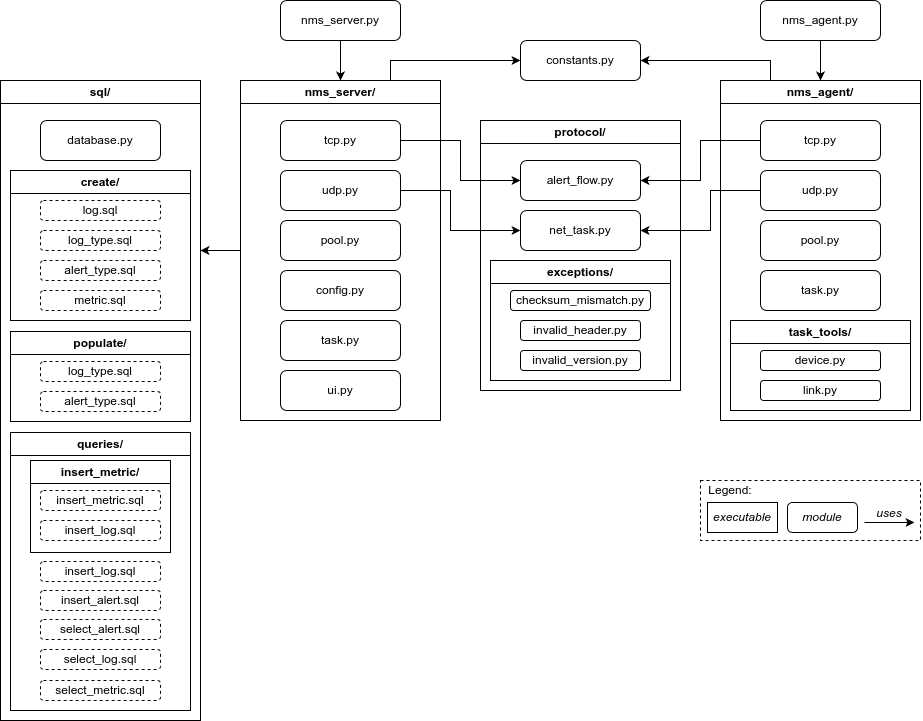
\includegraphics[width=\textwidth]{img/architecture.png}
    \captionof{figure}{Arquitetura da solução \textit{Network Monitoring System}}
    \label{fig:architecture}
\end{minipage}

%===============================================================================
% END ARQUITETURA DA SOLUÇÃO
%===============================================================================

%===============================================================================
% BEGIN ESPECIFICACÕES DOS PROTOCOLOS APLICACIONAIS
%===============================================================================

\newgeometry{top=0cm}

\chapter{Especificações dos Protocolos Aplicacionais}

\section{\textit{AlertFlow}}

O protocolo \textit{AlertFlow}, operado sobre o TCP, foi desenvolvido para a
comunicação de alertas de
agentes para o servidor, sendo assim utilizado monodirecionalmente. O envio de
alertas ocorre quando certas condições de monitorização definidas são excedidas,
sendo estas previamente indicadas pelo servidor, via o protocolo \textit{NetTask}.
Este protocolo é orientado à conexão, ou seja, cada vez que um agente envia um alerta,
é estabelecida uma nova conexão TCP com o servidor, sendo esta terminada após o envio
da mesma.

\subsection{Formato de Cabecalho e Descrição de Campos}

\begin{minipage}{\textwidth}
    \centering
    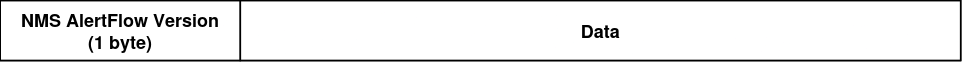
\includegraphics[width=\textwidth]{img/alertflow_header.png}
    \captionof{figure}{Formato do cabeçalho do protocolo \textit{AlertFlow}}
    \label{fig:alertflow_message_format}
\end{minipage}

\begin{itemize}
    \item \textbf{\textit{NMS AlertFlow Version}} (1 \textit{byte}): versão do protocolo,
        para assegurar a compatibilidade de versões entre o servidor e os agentes;
    \item \textbf{\textit{Data/Payload}} (n \textit{bytes}): carga útil da mensagem com
        tamanho variável. Utiliza a encodificação \textit{UTF-8}, com um formato JSON
        para a transmissão de dados.
\end{itemize}

\subsection{Descrição de Funcionalidades}

\textbf{Compatibilidade de Versões}

A compatibilidade de versões é garantida através do campo \textit{NMS AlertFlow Version}
do cabeçalho da mensagem, permitindo a identificação da versão do protocolo entre o
servidor e os agentes. Se a versão do protocolo do emissor for diferente da versão do
recetor, é apresentada uma mensagem de erro com as diferentes versões. Esta é meramente
indicativa à qual o formato usado nos dados da mensagem.

\loadgeometry{default}
\clearpage

\section{\textit{NetTask}}

O protocolo \textit{NetTask} é essencial para a funcionalidade harmonizada do
\textbf{\textit{Network Monitoring System}}, sendo este usado para a maioria
das comunicações entre o servidor e os agentes, tais como, a primeira conexão de
um agente ao servidor, o envio de tarefas pelo servidor, o envio de resultados
de tarefas pelos agentes, e a terminação de conexões nos dois sentidos, sendo
um protocolo orientado aos datagramas.

Como este opera em cima da camada de transporte UDP, o protocolo \textit{NetTask}
foi desenvolvido para ser robusto e adaptável a condições adversas de rede,
garantindo a entrega fiável e integral de mensagens, sobretudo em rotas deterioradas,
com perdas ou duplicação de pacotes, latências elevadas e taxas de débito variáveis.

Para combater tais adversidades, o protocolo aplicacional \textit{NetTask}
responsabiliza-se pelas funcionalidades que serão exploradas no seguinte
subcapítulo \ref{subsec:nt_desc_funcionalidades}.

Nos próximos subcapítulos, serão detalhadas as especificações do protocolo,
nomeadamente o formato do cabeçalho e descrição dos respetivos campos,
descrição de funcionalidades e diagramas de sequência que ilustram o
comportamento do protocolo em situações normais e adversas.

\subsection{Formato de Cabeçalho e Descrição de Campos}

\begin{minipage}{\textwidth}
    \centering
    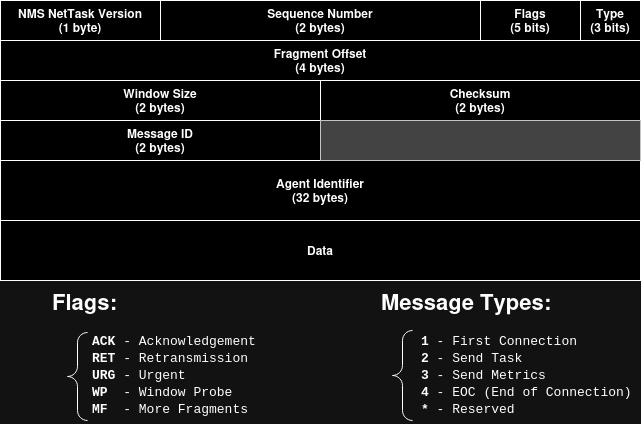
\includegraphics[width=\textwidth]{img/nettask_header.png}
    \captionof{figure}{Formato do cabeçalho do protocolo \textit{NetTask}}
    \label{fig:nettask_message_format}
\end{minipage}

\begin{itemize}
    \item \textbf{\textit{NMS NetTask Version}} (1 \textit{byte}):  versão do protocolo,
        para assegurar a compatibilidade de versões entre o servidor e os agentes;
    \item \textbf{\textit{Sequence Number}}     (2 \textit{bytes}): número de sequência da mensagem,
        para a ordenação de pacotes, deteção de pacotes duplicados e identificação de \textit{acknowledgements};
    \item \textbf{\textit{Flags}}               (5 \textit{bits}):  \textit{flags} de controlo:
        \begin{itemize}
           \item [\textbf{\textit{ACK}}] (1º \textit{bit}): \textit{Acknowledgement}, utilizado para confirmar a receção de pacotes;
           \item [\textbf{\textit{RET}}] (2º \textit{bit}): \textit{Retransmission}, indica que o pacote é uma retransmissão;
           \item [\textbf{\textit{URG}}] (3º \textit{bit}): \textit{Urgent}, indica que a mensagem é urgente, esquivando-se de mecanismos de controlo de fluxo;
           \item [\textbf{\textit{WP}} ] (4º \textit{bit}): \textit{Window Probe}, utilizado para o controlo de fluxo;
           \item [\textbf{\textit{MF}} ] (5º \textit{bit}): \textit{More Fragments}, para (des)fragmentação de pacotes.
        \end{itemize}
    \item \textbf{\textit{Type}}                (3 \textit{bits}): tipo da mensagem:
        \begin{itemize}
            \item [\textbf{0}]  \textbf{\textit{Undefined}}:               mensagem indefinida, utilizada
                para testes ou quando nenhum tipo de mensagem é aplicável,
                por exemplo no envio de \textit{window probes};
            \item [\textbf{1}]  \textbf{\textit{First Connection}}:        primeira conexão de um agente ao servidor;
            \item [\textbf{2}]  \textbf{\textit{Send Tasks}}:              envio de tarefas pelo servidor;
            \item [\textbf{3}]  \textbf{\textit{Send Metrics}}:            envio de resultados de tarefas pelos agentes;
            \item [\textbf{4}]  \textbf{\textit{EOC (End of Connection)}}: terminação de conexões nos dois sentidos;
            \item [\textbf{*}] \textbf{\textit{Reserved}}:                reservado para futuras extensões (de 5 a 7);
        \end{itemize}
    \item \textbf{\textit{Window Size}}        (2 \textit{bytes}): indica o tamanho da janela de receção,
        para o controlo de fluxo;
    \item \textbf{\textit{Checksum}}           (2 \textit{bytes}): soma de verificação da mensagem,
        para a deteção de erros;
    \item \textbf{\textit{Message Identifier}} (2 \textit{bytes}): identificador da mensagem,
        utilizado para a desfragmentação e ordenação de pacotes;
    \item \textbf{\textit{Agent Identifier}}   (32 \textit{bytes}): identificador do agente,
        podendo este ser recetor ou emissor da mensagem;
    \item \textbf{\textit{Data/Payload}}       (n \textit{bytes}): carga útil da mensagem com
        tamanho variável, contendo a informação a ser transmitida nas mensagens do tipo
        \textit{Send Tasks} e \textit{Send Metrics}. Utiliza a encodificação \textit{UTF-8},
        com um formato JSON para a transmissão de dados.
\end{itemize}

\clearpage

\subsection{Descrição de Funcionalidades}
\label{subsec:nt_desc_funcionalidades}

\textbf{Retransmissão de Pacotes Perdidos}

A retransmissão de pacotes perdidos é efetuada quando o emissor não recebe um
\textit{acknowledgement} de um pacote enviado, após um determinado intervalo de
tempo. Para a concretização desta funcionalidade, o emissor guarda todos os pacotes
enviados em memória, reenviando os pacotes não confirmados após o intervalo de tempo
definido no fichero \texttt{constants.py} sobre a nomenclatura \texttt{RETRANSMIT\_SLEEP\_TIME}.
Os pacotes mantém o cabeçalho original, sendo apenas ativada a \textit{flag RET}.


\textbf{(Des)Fragmentação e Ordenação de Pacotes}

A fragmentação de pacotes ocorre quando a carga útil da mensagem excede o tamanho
máximo permitido, sendo este tamanho predefinido para 1500 \textit{bytes}, no
ficheiro \texttt{constants.py} sobre a nomenclatura \texttt{BUFFER\_SIZE},
uma vez que este é o valor máximo para o \textit{Maximum Transmission Unit} (MTU).

Na fragmentação de pacotes, os dados da mensagem (campo \textit{Data}) são divididos em fragmentos,
de forma a que, com adição do cabeçalho, o tamanho total do pacote não exceda o tamanho
máximo permitido. Os primeiros fragmentos são marcados com a \textit{flag MF},
com exceção do último fragmento, indicando que não existem mais fragmentos a serem enviados.
Para a identificação dos fragmentos, é atribuído um \textit{Message Identifier} único, sendo
este igual ao número de sequência do primeiro fragmento. Os números de sequência dos fragmentos
são incrementados de forma sequencial.

Na desfragmentação, o recetor mantém em memória os fragmentos recebidos, cada pacote
recebido é guardado em um \textit{array} caso seja fragmentado. Para identificar
se um pacote é ou não um fragmento, é verificado se a \textit{flag MF} está desativada
e se o \textit{Message Identifier} é igual ao número de sequência do pacote. Se tal
não se verificar, o pacote é guardado em memória até que todos os fragmentos sejam
recebidos, ou seja, devem existir todos os fragmentos tal que o seu número de sequência
esteja entre os seus \textit{Message Identifiers} e o número de sequência do último fragmento.
Este procedimento garante que a mensagem é desfragmentada apenas quando todos os
fragmentos são recebidos, uma vez que a ordem de chegada destes não é garantida.

Uma vez que todos os fragmentos são recebidos, estes são ordenados pelo número de
sequência e os dados da mensagem são concatenados para formar a mensagem original.

O campo \textit{Message Identifier} permite que fragmentos de diferentes mensagens
sejam distinguidos, garantindo a integridade dos pacotes reconstruídos.


\clearpage

\textbf{Deteção e Manuseamento de Pacotes Duplicados}

A deteção e manuseamento de pacotes duplicados, tal como na (des)fragmentação
e ordenação de pacotes, recorre ao \textit{Sequence Number} da mensagem.
O recetor mantém um registo dos números de sequência de pacotes recebidos para a
deteção de pacotes duplicados, descartando pacotes que já tenham sido recebidos anteriormente, e
reenviando um \textit{acknowledgement} ao emissor para confirmar a receção do pacote
de forma a evitar futuras retransmissões desnecessárias.


\textbf{Deteção de Erros}

A deteção de erros é efetuada através da soma de verificação da mensagem (\textit{Checksum}),
calculada com base no cabeçalho e na carga útil da mensagem. O recetor, ao receber
um pacote, calcula a soma de verificação e compara-a com a recebida. Se a soma de
verificação calculada for diferente da recebida, o pacote é descartado, e o emissor
uma vez que não recebe um \textit{acknowledgement} reenviará o pacote.


\textbf{Compatibilidade de Versões}

A compatibilidade de versões é garantida através do campo \textit{NMS NetTask Version} do cabeçalho
da mensagem, permitindo a identificação da versão do protocolo entre o servidor e os agentes. Se a
versão do protocolo do emissor for diferente da versão do recetor, é apresentada uma mensagem de erro
com as diferentes versões. Uma possível alteração na implementação seria descartar a mensagem, evitando
possíveis incompatibilidades e erros, contudo, a decisão foi manter a mensagem de erro e tentar processar
o pacote, uma vez que a diferença de versões pode não impedir uma troca sem conflitos, deste modo, não
se sobrecarrega a largura de banda com múltiplas retransmissões de pacotes.


\textbf{Controlo de Fluxo}

O controlo de fluxo é efetuado através do tamanho da janela de receção (\textit{Window Size}),
indicando ao emissor o número de pacotes que o recetor pode receber sem congestionar a ligação.
O valor inicial da janela de receção é definido no ficheiro \texttt{constants.py} sobre a nomenclatura
\texttt{INITIAL\_WINDOW\_SIZE}, sendo este valor de 32 pacotes. O emissor, ao enviar um pacote, indica
a sua janela de receção, sendo esta referente à quantidade de espaço disponível na sua lista de pacotes
por desfragmentar e ordenar, uma vez que na implementação atual, é criada uma \textit{thread} para processar
pacotes recebidos, então apenas os pacotes fragmentados são guardados em memória, servindo estes para a indicação
do tamanho da janela de receção.
Quando a janela de receção do recetor é menor ou igual a zero, o emissor, antes de enviar pacotes, aguarda até que essa incremente,
de forma a não congestionar a rede e o recetor. Para esta medição dos \textit{window sizes}
dos recetores, é, posteriormente, criada uma \textit{thread} responsável por enviar \textit{window probes} aos mesmos
com \textit{window sizes} menores ou iguais a zero, de forma a que estes respondam com a sua janela de receção.


\clearpage

\subsection{Diagramas de Sequência}

\textbf{\textit{First Connection}}

\begin{minipage}{\textwidth}
    \centering
    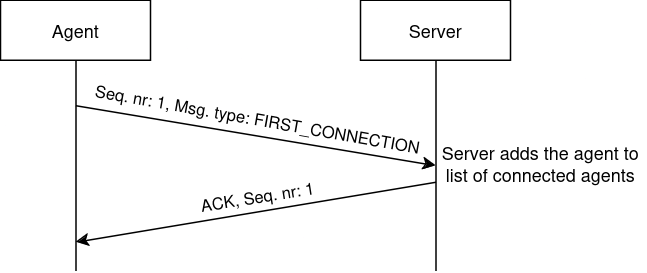
\includegraphics[width=0.7\textwidth]{img/sequence_diagrams/first_connection.png}
    \captionof{figure}{Diagrama de sequência do protocolo \textit{NetTask} - \textit{First Connection}}
    \label{fig:nt_first_connection}
\end{minipage}

\vspace{1cm}

\textbf{\textit{End of Connection (EOC)}}

\begin{minipage}{\textwidth}
    \centering
    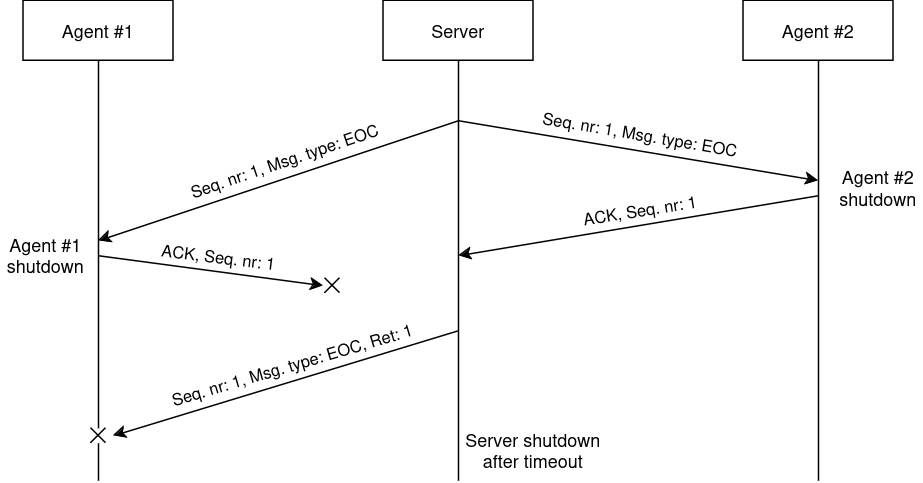
\includegraphics[width=\textwidth]{img/sequence_diagrams/end_of_connection.png}
    \captionof{figure}{Diagrama de sequência do protocolo \textit{NetTask} - \textit{End of Connection}}
    \label{fig:nt_end_of_connection}
\end{minipage}

Neste exemplo, o servidor é interrompido, sendo enviado um pacote \textit{EOC} para
todos os agentes, terminando todas as execuções. O mesmo pode ser feito quando um agente
é interrompido, sendo enviado um pacote \textit{EOC} para o servidor, e este remove
o agente da lista de agentes conectados.

Note que, em rotas deterioradas, a mensagem de \textit{End of Connection} pode não ser recebida,
então é necessário determinar um tempo para um \textit{timeout} adequado as condições da rede,
de forma a garantir a terminação da conexão com sucesso.

\clearpage
\textbf{Retransmissão, Manuseamento de Pacotes Duplicados, Desfragmentação, Ordenação e Deteção de Erros}

\begin{minipage}{\textwidth}
    \centering
    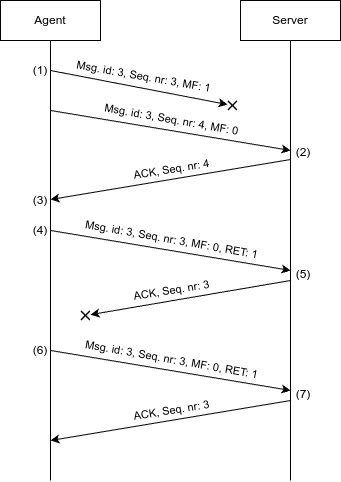
\includegraphics[width=0.45\textwidth]{img/sequence_diagrams/ret_dup_frag_ord_error.png}
    \captionof{figure}{Diagrama de sequência do protocolo \textit{NetTask} - Retransmissão, Manuseamento de Pacotes Duplicados, Desfragmentação, Ordenação e Deteção de Erros}
    \label{fig:nt_ret_dup_frag_ord_error}
\end{minipage}

\begin{enumerate}
    \item O agente envia uma métrica, com dados superiores ao \texttt{BUFFER\_SIZE}, subtraído do \textit{header size},
    sendo este fragmentado em dois pacotes;
    \item O servidor recebe o pacote, e como o \textit{Message Id} é diferente do \textit{Sequence Number}, deduz que
    faltam mais fragmentos, adicionando-o ao seu \textit{buffer} de pacotes a desfragmentar, e envia o ACK;
    \item O agente remove o pacote de número de sequência 4 da lista de pacotes por retransmitir;
    \item O agente, após aguardar \texttt{RETRANSMIT\_SLEEP\_TIME} segundos, retransmite o pacote não \textit{acknowledged};
    \item O servidor possui todos os fragmentos, ordena e desfragmenta os mesmos, guardando a métrica na base de dados.
    Seguidamente, envia o ACK, que será perdido;
    \item O agente, ao não receber o ACK, retransmite o pacote pela segunda vez, que, pela sua rota, sofre de alterações
    no seu conteúdo;
    \item O servidor, ao receber o pacote, calcula o \textit{checksum} e verifica que é diferente do expectado, descartando
    o pacote. Como tal, não envia um ACK;
    \item O agente, ao não receber o ACK, retransmite o pacote novamente;
    \item O servidor descarta o pacote duplicado, pois, no passo (5), já tinha guardado o número de sequência 3.
    O servidor reenvia o ACK para evitar retransmissões desnecessárias.
\end{enumerate}

\clearpage

\textbf{Controlo de Fluxo}

\begin{minipage}{\textwidth}
    \centering
    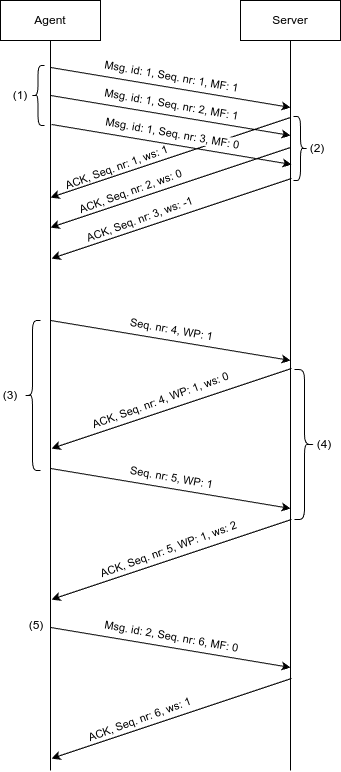
\includegraphics[width=0.4\textwidth]{img/sequence_diagrams/flux_control.png}
    \captionof{figure}{Diagrama de sequência do protocolo \textit{NetTask} - Controlo de Fluxo}
    \label{fig:nt_flux_control}
\end{minipage}

O agente pretende enviar dois pacotes, sendo o primeiro de grande porte, num curto espaço de tempo. Este primeiro tem que ser
fragmentado e enviado em três pacotes distintos \textbf{(1)}. Entretanto, a \textit{window size} encontra-se a dois.
O servidor, ao receber os pacotes, encarrega-se de enviar os respetivos ACKs, atualizando a sua \textit{window size}, até que, no terceiro
pacote, ela encontra-se a -1 \textbf{(2)}. O agente necessitava enviar mais um pacote, porém, a \textit{window size} é inferior a zero,
então sabe que o servidor tem o \textit{buffer} cheio, pelo que envia \textit{window probes} \textbf{(3)} para o servidor
até este lhe indicar que a sua \textit{window size} voltou a ser superior a zero \textbf{(4)}. Posto isto, o agente pode finalmente enviar
o pacote em falta \textbf{(5)}.


%===============================================================================
% END PROTOCOLOS APLICACIONAIS
%===============================================================================

%===============================================================================
% BEGIN IMPLEMENTAÇÃO
%===============================================================================

\chapter{Implementação}

\section{Parâmetros dos Executáveis}

\subsection{\texttt{nms\_server.py}}

\begin{lstlisting}[
    language=,
    caption={Parâmetros do executável \textit{nms\_server.py}},
    label={lst:nms_server_params},
    numbers=none
]
$ ./nms_server.py --help
usage: nms_server.py [-h] [-c CONFIG] [-v]

Network Management System Server

options:
  -h, --help            show this help message and exit
  -c CONFIG, --config CONFIG
                        Configuration file path
  -v, --verbose         Enable verbose output
\end{lstlisting}

\subsection{\texttt{nms\_agent.py}}

\begin{lstlisting}[
    language=,
    caption={Parâmetros do executável \textit{nms\_agent.py}},
    label={lst:nms_agent_params},
    numbers=none
]
$ ./nms_agent.py --help
usage: nms_agent.py [-h] [-s SERVER] [-v]

Network Management System Agent

options:
  -h, --help            show this help message and exit
  -s SERVER, --server SERVER
                        Server IP
  -v, --verbose         Enable verbose output
\end{lstlisting}

\section{Ficheiro de Configuração}

O ficheiro de configuração permite a definição de tarefas aos agentes pelo servidor.
Este é carregado no início da execução do servidor, e é enviado a cada agente, aquando
da sua conexão, as tarefas as quais este deve executar.
O sistema desenvolvido suporta as seguintes métricas e alertas:

\begin{itemize}
    \item \textbf{Métricas de dispositivo}:
    \begin{itemize}
        \item \textbf{\textit{CPU Usage}}: percentagem de utilização da CPU;
        \item \textbf{\textit{RAM Usage}}: percentagem de utilização da memória RAM;
        \item \textbf{\textit{Interfaces Stats}}: número de pacotes por segundo,
            para cada interface de rede definida.
    \end{itemize}
    \item \textbf{Métricas de rede}:
    \begin{itemize}
        \item \textbf{\textit{Bandwidth}}: consumo de largura de banda, em \textit{Mbps} (\textit{iperf} via TCP);
        \item \textbf{\textit{Jitter}}: variação de atraso, em milissegundos (\textit{iperf} via UDP, \textit{ping});
        \item \textbf{\textit{Packet Loss}}: percentagem de pacotes perdidos (\textit{iperf} via UDP, \textit{ping});
        \item \textbf{\textit{Latency}}: atraso entre o envio e a receção de pacotes, em milissegundos (\textit{ping}).
    \end{itemize}
    \item \textbf{Alertas}: aquando os valores obtidos excedem os limites definidos.
    \begin{itemize}
        \item \textbf{\textit{CPU Usage}};
        \item \textbf{\textit{RAM Usage}};
        \item \textbf{\textit{Interfaces Stats}};
        \item \textbf{\textit{Packet Loss}};
        \item \textbf{\textit{Jitter}}.
    \end{itemize}
\end{itemize}

Neste ficheiro, é possível definir os parâmetros de utilização de cada ferramenta usada no cálculo das métricas,
por exemplo, no caso do \texttt{iperf3}, é possível definir a duração do teste, a camada de transporte, se tal é
\textit{server} ou \textit{client}, entre outros. Estes parâmetros são utilizados por tarefa, o que permite a
diferentes agentes executarem o mesmo teste com diferentes parâmetros.

Outra consideração importante na utilização do \texttt{iperf3} é a necessidade de
definir as tarefas de ambos os agentes, os quais em modo cliente ou servidor,
de forma a que seja possível executar o teste.

\section{Bibliotecas Utilizadas}

Para a implementação do \textbf{\textit{Network Monitoring System}}, foram utilizadas
as seguintes bibliotecas \textit{Python}:

\begin{itemize}
    \item \textbf{\texttt{socket}}: para a comunicação entre o servidor e os agentes,
    permitindo a troca de mensagens entre os sistemas, tanto em TCP como em UDP;
    \item \textbf{\texttt{threading}}: para a execução \textit{multi threading} de tarefas, servidores TCP e UDP,
    retransmições de pacotes, entre outros, permitindo multiprocessamento a ambos os agentes como o servidor;
    \item \textbf{\texttt{json}}: para a codificação e descodificação de \textit{payloads} de pacotes em formato JSON;
    \item \textbf{\texttt{psutil}}: para a recolha de métricas de desempenho dos dispositivos,
    permitindo a obtenção de informações sobre a utilização da CPU, memória RAM e interfaces de rede;
    \item \textbf{\texttt{iperf3}}: \textit{iperf wrapper} para a execução de testes de largura de banda,
    \textit{jitter} e \textit{packet loss}, permitindo a obtenção facilitada desses dados aquando
    o \textit{iperf} é executado como cliente;
    \item \textbf{\texttt{subprocess}}: utilizado para correr os comando nativos \textit{ping} e \textit{iperf3} (modo servidor),
    permitindo obter o \textit{return code}, \textit{stdout} e \textit{stderr} do comando.
    \item \textbf{\texttt{matplotlib}}: para a criação de gráficos, permitindo a visualização
    das métricas recolhidas e a sua evolução ao longo do tempo.
\end{itemize}

\clearpage

\section{Detalhes Técnicos da Implementação}

\subsection{Definição de Constantes}

Ao longo da implementação, foram definidas várias constantes, que permitem a
configuração do sistema. Estas constantes são definidas no ficheiro \texttt{constants.py},
e são as seguintes:

\begin{itemize}
    \item \textbf{\texttt{ENCODING}}: a definição de codificação de mensagens, pré-definida como \textbf{\textit{UTF-8}},
    sendo esta configurável, para, por exemplo, \textit{ASCII}, \textit{ISO-8859-1}, entre outras;
    \item \textbf{\texttt{BUFFER\_SIZE}}: o tamanho máximo de um pacote, definido como \textbf{1500 \textit{bytes}},
    este, o valor máximo para o \textit{Maximum Transmission Unit} (MTU) de uma rede Ethernet;
    \item \textbf{\texttt{SO\_NO\_CHECK}}: este valor permite desativar o cálculo do \textit{checksum} em
    pacotes UDP, permitindo um controlo de erros personalizado;
    \item \textbf{\texttt{RETRANSMIT\_SLEEP\_TIME}}: intervalo de tempo, em segundos, para retransmitir pacotes não confirmados.
    Definiu-se como \textbf{5 segundos}, permitindo uma rápida recuperação de pacotes perdidos sem causar sobrecarga excessiva na rede.
    A definição deste valor teve em conta que a retransmissão de pacotes precisa de um tempo de resposta curto para garantir
    o desempenho, porém, não tão curto como, por exemplo, nos serviços de \textit{streaming}, onde a latência é crítica.
    Manter este valor significamente maior reduz a sobrecarga computacional e de tráfego de rede, sendo ótimo para a aplicação desenvolvida;
    \item \textbf{\texttt{INITIAL\_WINDOW\_SIZE}}: o \textit{window size} inicial foi definido como \textbf{32 pacotes}.
    Este valor é suficiente para lidar com tráfego usual da aplicação, sem causar congestionamento na rede;
    \item \textbf{\texttt{WINDOW\_PROBE\_SLEEP\_TIME}}: intervalo de tempo, em segundos, antes de enviar \textit{window probes}
    a agentes com \textit{window sizes} menores ou iguais a zero.
    Definiu-se como \textbf{5 segundos}, permitindo uma verificação regular da janela de receção sem causar sobrecarga excessiva na rede;
    \item \textbf{\texttt{EOC\_ACK\_TIMEOUT}}: tempo máximo de espera, em segundos, para o recebimento de confirmações de término de conexão.
    O intervalo foi definido como três vezes o tempo de retransmissão para garantir três tentativas de retransmissão antes de encerrar a conexão.
\end{itemize}

\subsection{Base de Dados}

A base de dados foi implementada em \textit{MySQL}, onde se realizou a criação das tabelas,
bem como o seu povoamento e \textit{queries} para a obtenção e inserção de \textit{logs},
métricas e alertas. Estes ficheiros \texttt{sql} são posteriormente utilizados no módulo
\texttt{database.py} para as respetivas operações. O servidor, ao receber as métricas, alertas
e novas conexões, guarda estes dados na base de dados, permitindo a análise e visualização
dos mesmos.

\begin{minipage}{\textwidth}
    \centering
    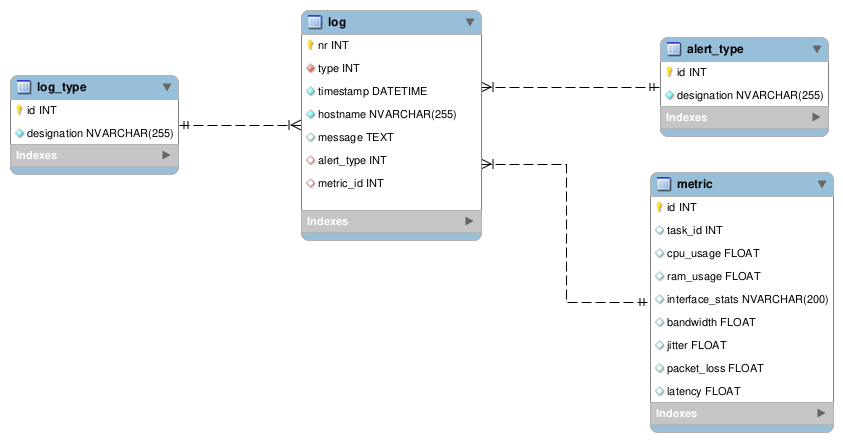
\includegraphics[width=\textwidth]{img/db.png}
    \captionof{figure}{Base de Dados do \textit{Network Monitoring System}}
    \label{fig:database}
\end{minipage}

\clearpage

\subsection{Análise Gráfica de Métricas}

Para a funcionalidade de análise gráfica de métricas, foi criado o executável
\texttt{analysis.py} que, após a recolha de métricas da base de dados, permite
a criação e visualização de gráficos. Este, permite a visualização das seguintes
seis métricas:

\begin{minipage}{.5\textwidth}
    \centering
    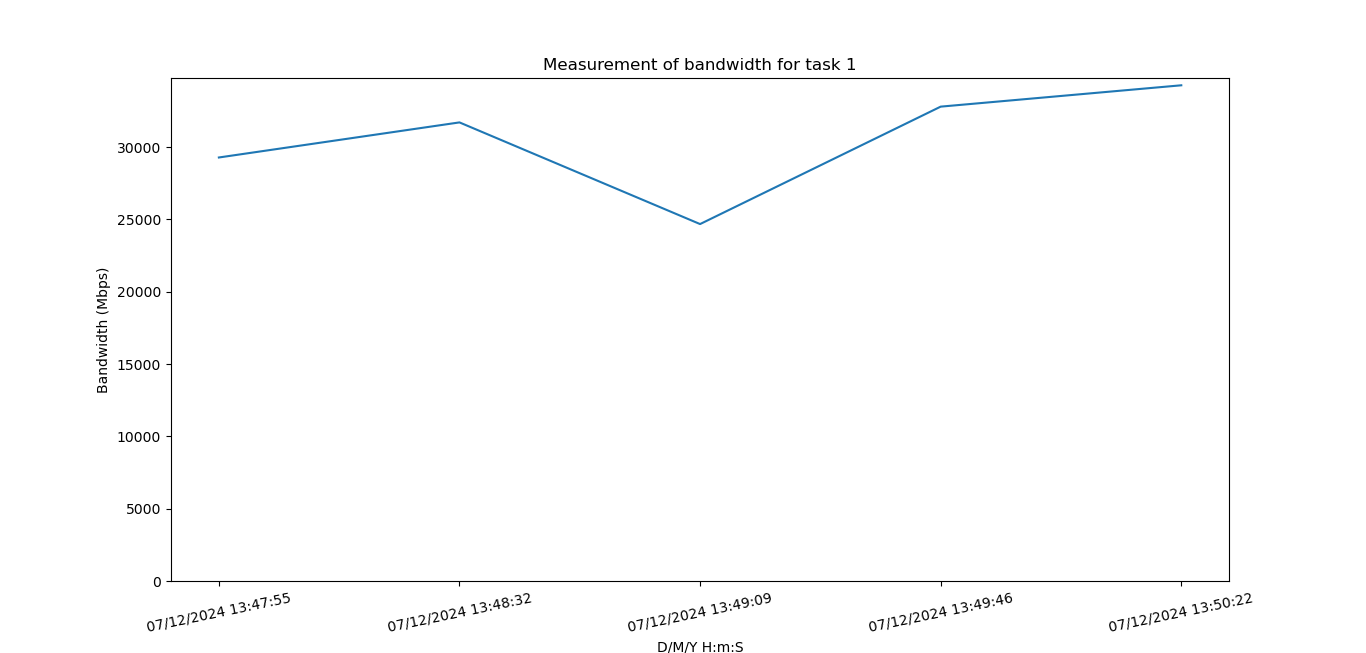
\includegraphics[width=\textwidth]{img/analysis/bandwidth.png}
    \captionof{figure}{\textit{Bandwidth}}
    \label{fig:bandwidth}
\end{minipage}
\hfill
\begin{minipage}{.5\textwidth}
    \centering
    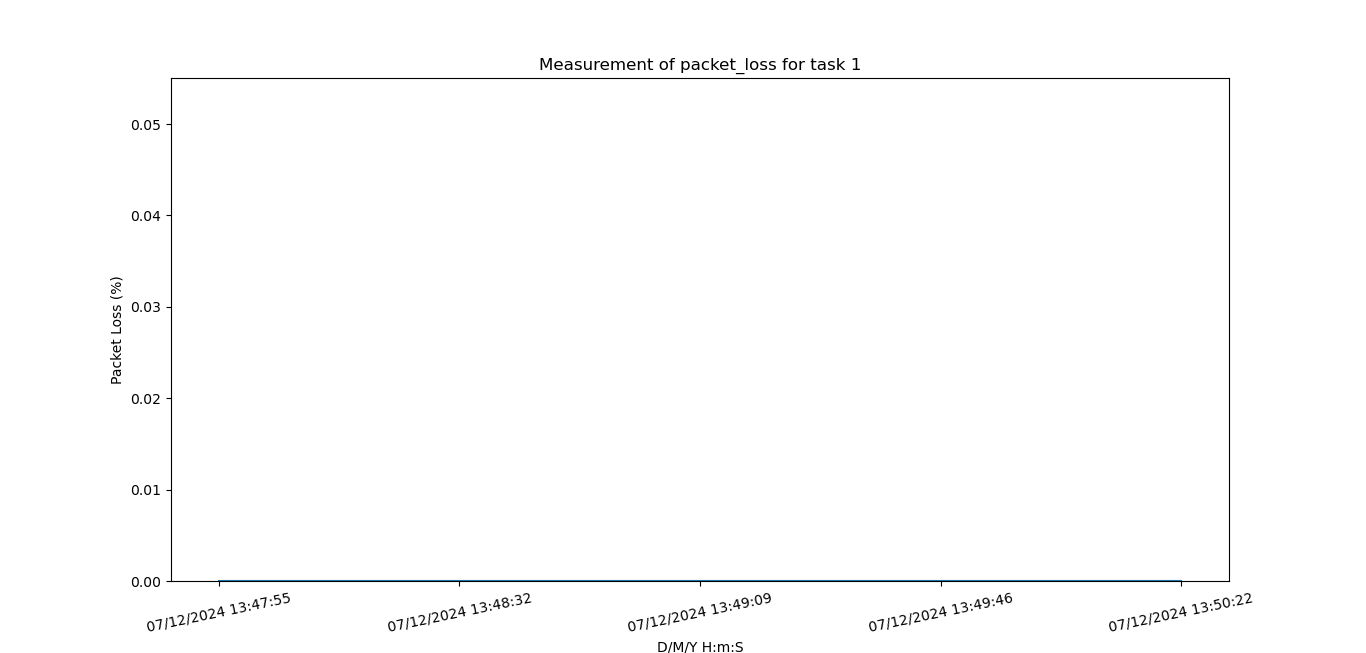
\includegraphics[width=\textwidth]{img/analysis/packet_loss.png}
    \captionof{figure}{\textit{Packet Loss}}
    \label{fig:packet_loss}
\end{minipage}

\begin{minipage}{.5\textwidth}
    \centering
    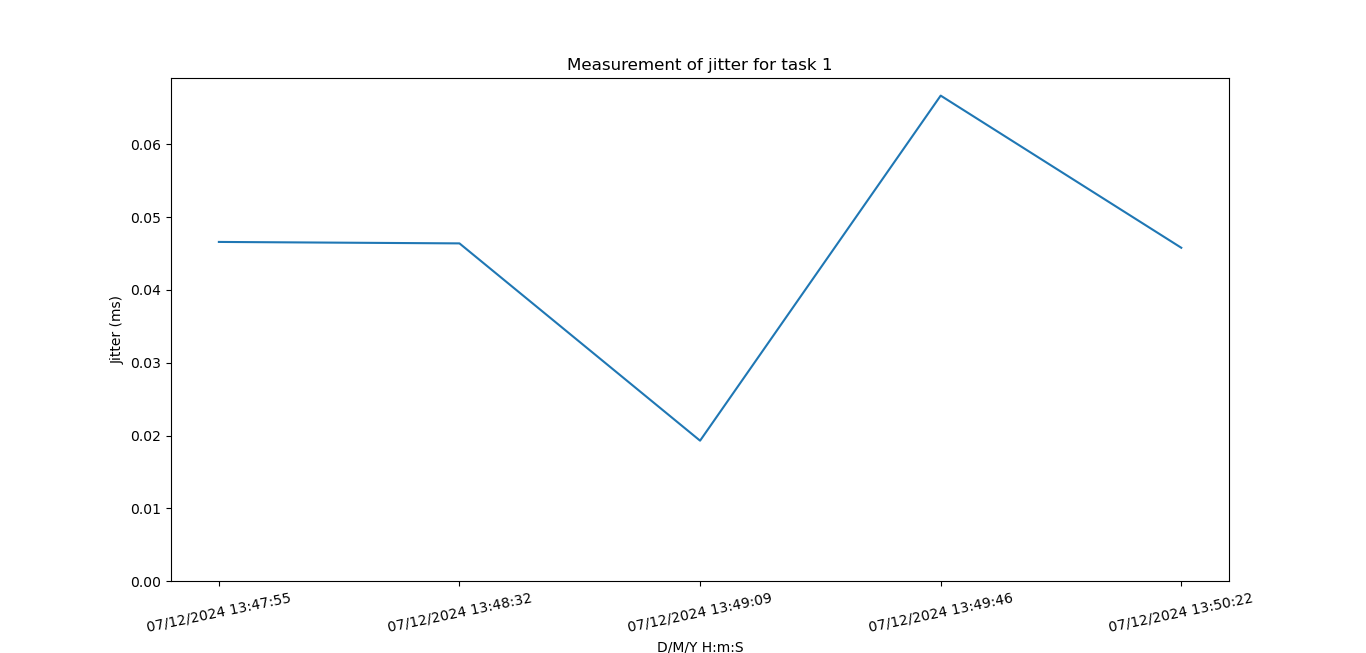
\includegraphics[width=\textwidth]{img/analysis/jitter.png}
    \captionof{figure}{\textit{Jitter}}
    \label{fig:jitter}
\end{minipage}
\hfill
\begin{minipage}{.5\textwidth}
    \centering
    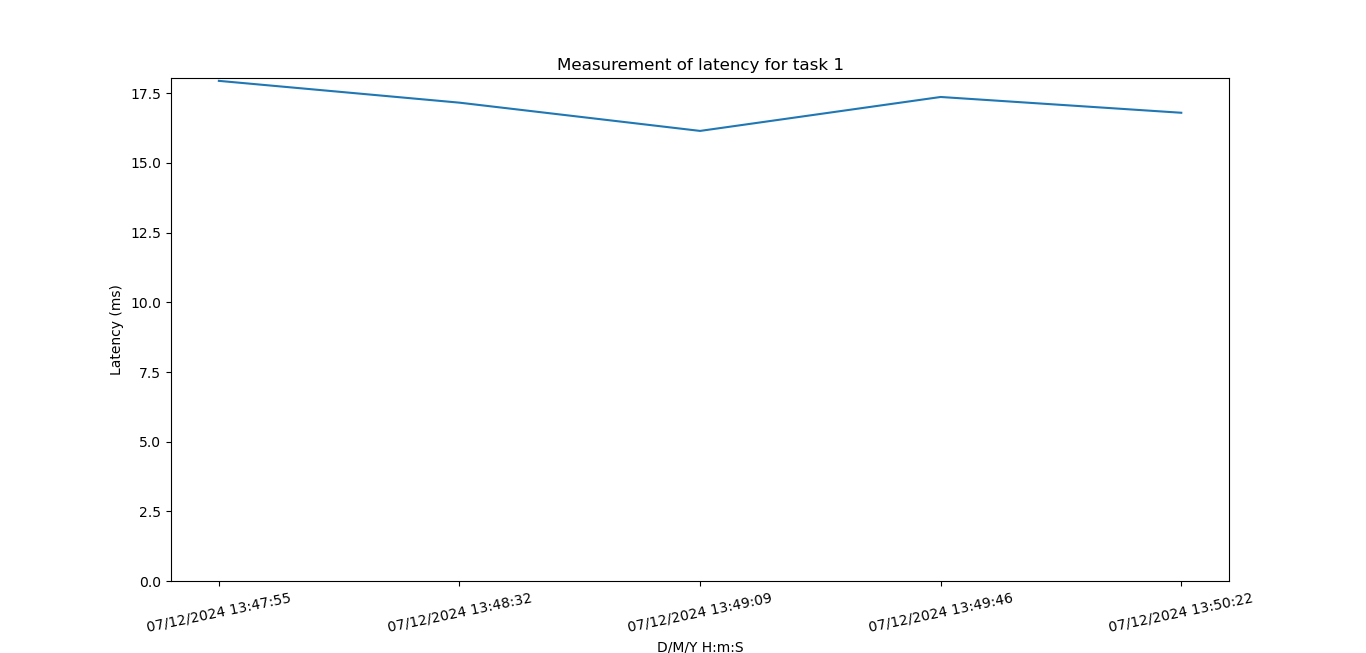
\includegraphics[width=\textwidth]{img/analysis/latency.png}
    \captionof{figure}{\textit{Latency}}
    \label{fig:latency}
\end{minipage}

\begin{minipage}{.5\textwidth}
    \centering
    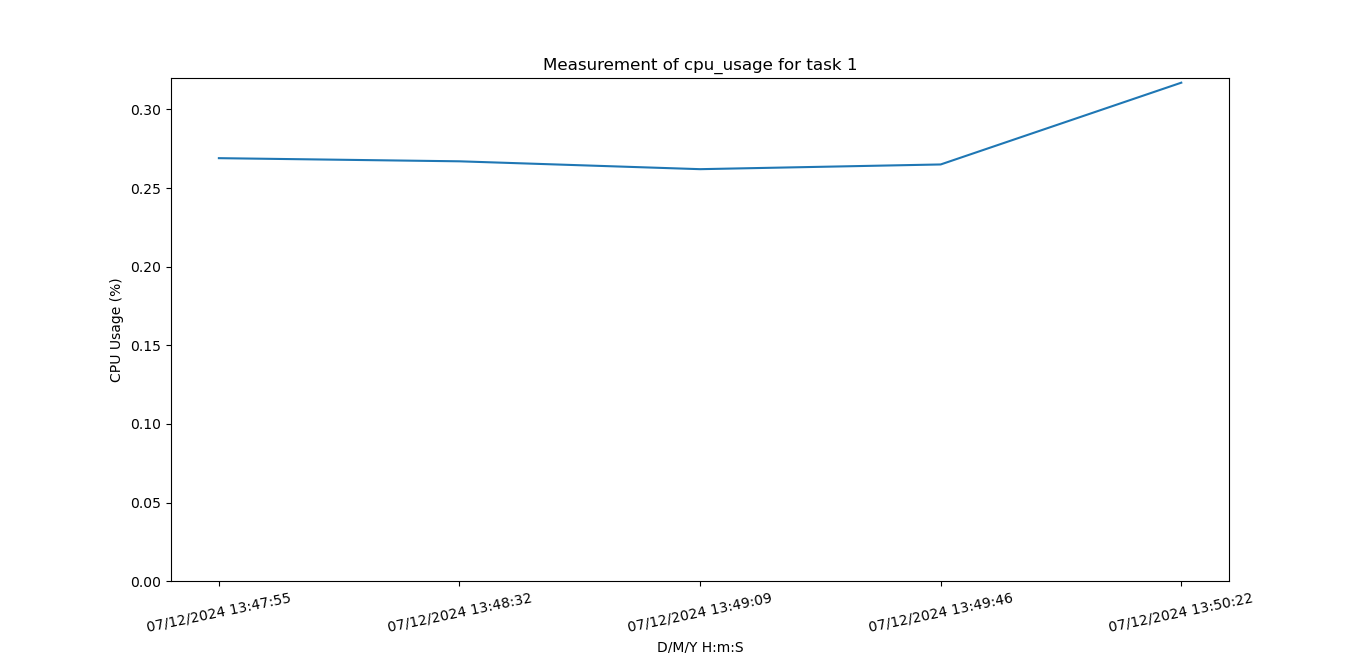
\includegraphics[width=\textwidth]{img/analysis/cpu_usage.png}
    \captionof{figure}{\textit{CPU Usage}}
    \label{fig:cpu_usage}
\end{minipage}
\hfill
\begin{minipage}{.5\textwidth}
    \centering
    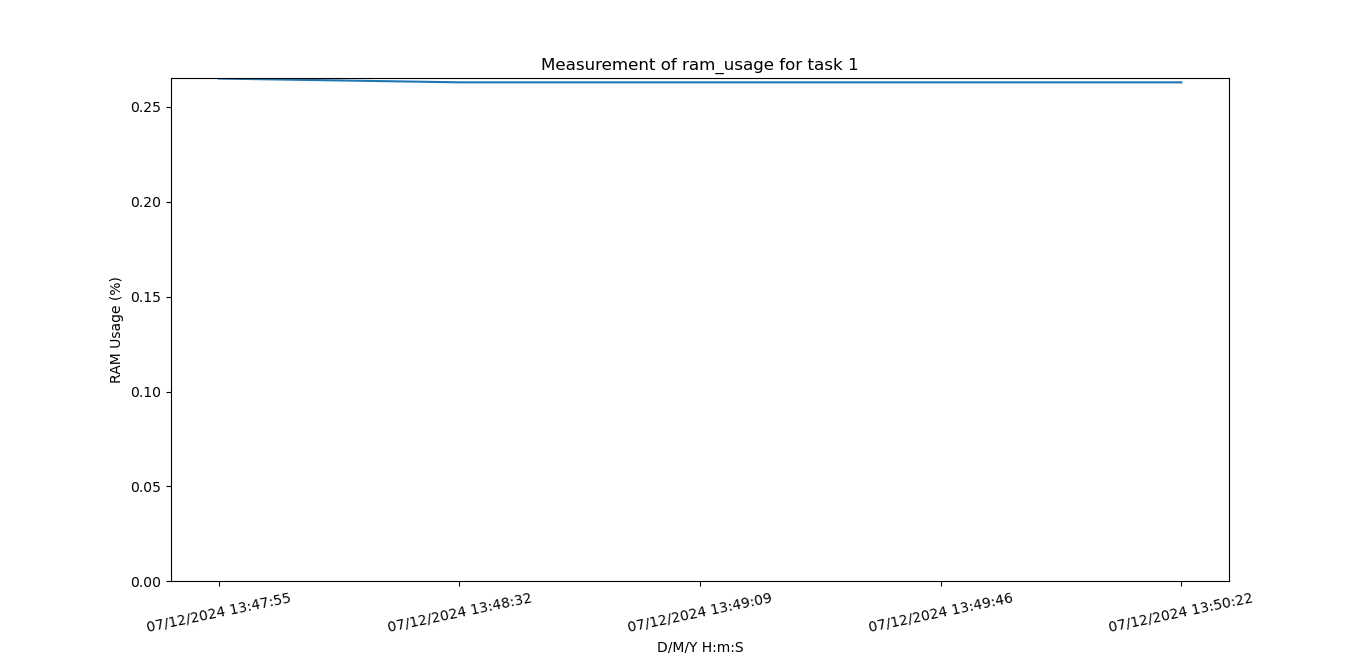
\includegraphics[width=\textwidth]{img/analysis/ram_usage.png}
    \captionof{figure}{\textit{RAM Usage}}
    \label{fig:ram_usage}
\end{minipage}


%===============================================================================
% END IMPLEMENTAÇÃO
%===============================================================================

%===============================================================================
% BEGIN TESTES E RESULTADOS
%===============================================================================

\chapter{Testes e Resultados}

\textcolor{red}{
    As demonstrações para situcoes normais e adversas, contam para este capítulo?
    Ou teremos de fazer testes mais específicos? \\
    Checksum, pacotes duplicados, retransmissão, defrag, controlo de fluxo, compatibilidade de versões...
}

%===============================================================================
% END TESTES E RESULTADOS
%===============================================================================

%===============================================================================
% BEGIN CONCLUSÕES E TRABALHO FUTURO
%===============================================================================

\chapter{Trabalho Futuro e Conclusões}

\section{Trabalho Futuro}

Como trabalho futuro, propõe-se a implementação das seguintes funcionalidades,
para uma maior completude do sistema desenvolvido:

\begin{itemize}
    \item \textbf{Encriptação de Mensagens}: adicionar encriptação de
    mensagens para garantir a confidencialidade e integridade dos dados transmitidos entre
    o servidor e os agentes, através da incorporação do uso de \textit{nonces}
    de forma a prevenir ataques \textit{Man-In-The-Middle}. Adicionalmente, uma forma de
    garantir a autenticidade das mensagens seria a utilização de uma autoridade de certificação
    para a emissão de certificados digitais para os agentes e o servidor, garantindo totalmente
    a confidencialidade, integridade, autenticação e não repúdio do originador.

    \item \textbf{Reatribuição de Tarefas em \textit{Runtime}}: permitir a reatribuição
    de tarefas em tempo de execução, para ajustar dinamicamente as tarefas dos agentes
    com base nas condições da rede e nos requisitos do sistema. Tal poderia ser implementado
    através do uso do identificador de uma tarefa, permitindo assim a sua adição e atualização,
    para além disso poderia ser adicionado ao \textit{User Interface} a possibilidade de
    adicionar tarefas, removê-las e atualizá-las. A nível protocolar, seria apenas necessário
    adicionar um novo tipo de mensagem, por exemplo, \textit{Remove Task}, que permitiria
    a remoção de tarefas. Para a opção de atualização de tarefas, apenas seria necessário
    que o agente atualizasse a tarefa com o mesmo identificador.
\end{itemize}

\clearpage

\section{Conclusões}

A realização deste projeto permitiu a aplicação prática dos conhecimentos adquiridos
durante o semestre na Unidade Curricular de \textbf{Comunicações por Computador},
nomeadamente no que diz respeito à conceção e implementação de protocolos aplicacionais
para a comunicação entre sistemas.

A implementação do \textbf{\textit{Network Monitoring System}} permitiu a integração de
vários conceitos e técnicas de comunicação, como a fragmentação de pacotes, retransmissão
de pacotes perdidos, controlo de fluxo, deteção de erros e ordenação de pacotes, garantindo
a fiabilidade e robustez do sistema.

Por conseguinte, o sistema desenvolvido demonstrou ser eficaz na monitorização e
análise de tráfego de rede, permitindo a recolha de métricas de
desempenho, a sua análise gráfica e a execução de tarefas de monitorização de forma
eficiente e fiável. A sua implementação permitiu a atualização da nossa perceção
do quanto damos por garantidos os protocolos de comunicação que utilizamos diariamente.

%===============================================================================
% END CONCLUSÕES E TRABALHO FUTURO
%===============================================================================

\end{document}
